\chapter{Software and Tools}
\label{existing_tech}

The existing system is based on the works from previous student projects and master theses. An overview of the present methods and tools will be needed to address some of the current objectives. In the following sections, introduces tools and functionality that plays a key role in this project

\section{Qt}

Qt is a cross-platform software development framework used for developing an application to various software and hardware platforms \cite{qt}. The framework is primarily used in regards to graphical applications since it has a range and support of tools for data presentation and interaction. Qt also provides GUI that emulate a native-looking interface. Application and libraries using Qt can be compiled by standard C++ compilers such as Clang, GCC and MinGW. 

The Qt Company provide extensive support and documentation of the framework so that for those with little knowledge of the framework can quickly get started. In addition, is it plenty of discussion forums for help and exchanging information among developers.


\section{GeoMod}

For underwater vehicles and their tools to work autonomous, the GeoMod software was developed as a platform for simulation and testing environment to handle real life assignments. The software was first developed by Professor Sven Fjeldaas at NTNU for this purpose. The development of the software has since then been a collaboration project by several students over the years. From the initial development till this day, substantial changes have been done such as porting between platforms and update of code to keep up with the latest Qt version.

(more) - limitation, analysis,functionality, underliggende krav...


\subsection{Model}
\label{chap:model}

\begin{figure}[ht]
    \centering
    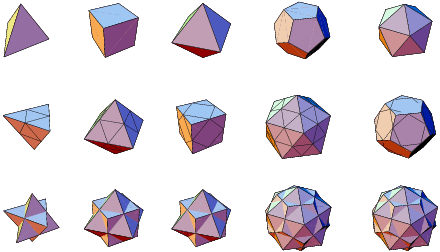
\includegraphics[height=5cm]{images/poly.png}
    \caption[Various type of polyhedrons \cite{polyhedrons}]{Various type of polyhedrons \cite{polyhedrons}}
    \label{fig:polyhedrons}
\end{figure}

Vehicles and tools are in GeoMod created of mathematical geometric models rendered as multiple composed polyhedrons. \Cref{fig:polyhedrons} illustrates how polyhedrons can form various types of shapes to create complex objects. GeoMod manages this by creating nodes with connected edges forming flat regions through the classes \textit{GeomNode} and \textit{GeomEdge}. The acquisition of the project included a few simple models, in addition to a model of a manipulator made from model parts that are linked together. These models, seen from \Cref{fig:viewport}, are used as a basis for the implementation of the control system. They are in the current state made in individual source files that are manually hardcoded in the software. 

\begin{figure}[ht]
    \centering
    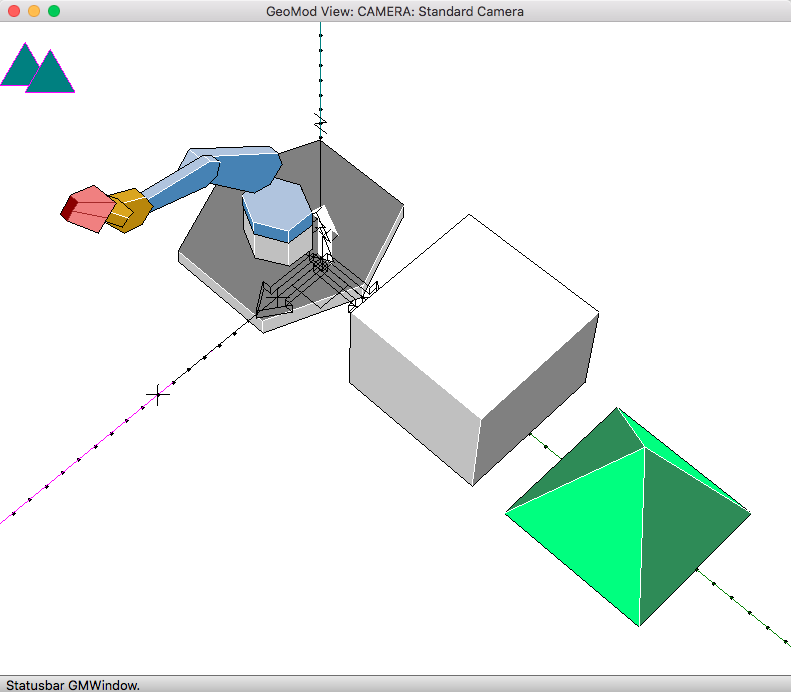
\includegraphics[height=8cm]{images/Models.png}
    \caption[The GeoMod viewport is showing a geometric model of a typical serial manipulator, pyramid and cube]{The GeoMod viewport is showing a geometric model of a typical serial manipulator, pyramid and cube.}
    \label{fig:viewport}
\end{figure}

During this project, there have been other students working parallel with the development of the software. Their assignment has, on the other hand, focused on using dynamic linking with the concern in this topic. The way it is today the code is statically linked as the program is created(compiled). The program has to be recompiled if there are changes and updates in the code or library. With dynamic linking, new models can be added during runtime that corresponds to how autonomous systems should work. This has to be taken into consideration when an implementation of a control system is based on how the models are being handled in the software.


\subsection{Model transformation}

\begin{figure}[ht]
    \centering
    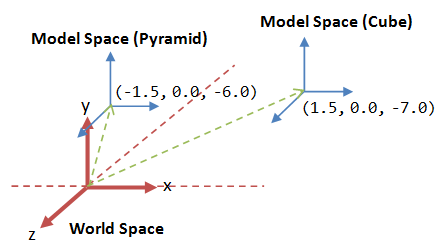
\includegraphics[height=5cm]{images/ModelSpace.png}
    \caption[Model transformation \cite{modelspace}]{Model transformation \cite{modelspace}}
    \label{fig:modelspace}
\end{figure}

Models in GeoMod consists each with a transformation group of the class \textit{TGroup}, which contains geometric information of the model in Cartesian coordinate system. The class consisted again of a basis that allows models to have their own coordinate system (model space). By setting an offset vector and orientation of the basis relative to the main coordinate system (world space) enables models to be moved and rotated in a three dimensional space (\Cref{fig:modelspace}). For the serial manipulator model, the same principle works on the joints. The model-parts are using an offset vector between the joint basis and the world space for position and orientation to create a linked model. Through subroutines can valid joints movement be calculated from their bases.

The models used in this project came with each a panel for movement when the software was handed over. These panels are very limited as it only has translation and rotation options along one of the three axes. In \Cref{fig:controlcube} shows the panel for the model named "cube" consisting of buttons in the X, Y and Z directions with respect to translation and rotation. Movement is done incrementally as the step value is determined beforehand and hard-coded. 

The models used in this project came with each a panel for movement when the software was handed over. These panels are very limited as it only has translation and rotation options along one of the three axes. In \Cref{fig:controlcube} a panel for the model named "cube" is shown. It consists of buttons for X, Y and Z directions with respect to translation and rotation. Movement is done incrementally as the step value is determined beforehand and hard-coded. The panel also contains a functionality to save the sequence of motion of the model to repeat the same movement. Dejectedly, this feature has not yet been implemented in the currently given version of GeoMod. 

\begin{figure}[ht]
    \centering
    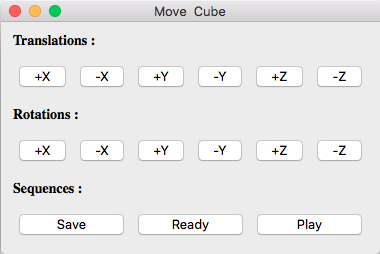
\includegraphics[height=5cm]{images/control_cube.png}
    \caption[Control panel for the cube model]{Control panel for the cube model}
    \label{fig:controlcube}
\end{figure}


\subsection{Paths}

In GeoMod a basic proof of concept for path created as a network, have been implemented by Martin Lygre Furevik in his master thesis, Spring 2016. In his work paths are implemented like models in GeoMod. As models are created with GeomNode and GeomEdge, paths are also formed by edges connected to nodes. Paths and models share many of the same properties and include many of the same features can be used on paths. This implies that paths can be moved and rotated like models as they also contain geometric data within a transformation group. A network of paths is made of a list of edges and nodes that count as linear or curved lines for guidance. 

The handed GeoMod version at the start of this project included a path object resemblance to a cube. Just like with dynamic linking, there is also another student working parallel with this project to manage creation and editing of paths at runtime.